%%%%%%%%%%%%%%%%%%%%%%%%%%%%%%%%%%%%%%%%%
% University/School Laboratory Report
% LaTeX Template
% Version 3.1 (25/3/14)
%
% This template has been downloaded from:
% http://www.LaTeXTemplates.com
%
% Original author:
% Linux and Unix Users Group at Virginia Tech Wiki 
% (https://vtluug.org/wiki/Example_LaTeX_chem_lab_report)
%
% License:
% CC BY-NC-SA 3.0 (http://creativecommons.org/licenses/by-nc-sa/3.0/)
%
%%%%%%%%%%%%%%%%%%%%%%%%%%%%%%%%%%%%%%%%%

%----------------------------------------------------------------------------------------
%	PACKAGES AND DOCUMENT CONFIGURATIONS
%----------------------------------------------------------------------------------------

\documentclass{article}

%\usepackage[version=3]{mhchem} % Package for chemical equation typesetting
%\usepackage{siunitx} % Provides the \SI{}{} and \si{} command for typesetting SI units
\usepackage{graphicx} % Required for the inclusion of images
%\usepackage{natbib} % Required to change bibliography style to APA
\usepackage{amsmath} % Required for some math elements 
\usepackage{float}
\usepackage{changepage}



\setlength\parindent{0pt} % Removes all indentation from paragraphs

%\renewcommand{\labelenumi}{\alph{enumi}.} % Make numbering in the enumerate environment by letter rather than number (e.g. section 6)

%\usepackage{times} % Uncomment to use the Times New Roman font

%----------------------------------------------------------------------------------------
%	DOCUMENT INFORMATION
%----------------------------------------------------------------------------------------

\title{Fundaments of HPC \\ Second Assignment} % Title

\author{Nicola \textsc{Domenis}} % Author name

\date{\today} % Date for the report

\begin{document}

\maketitle % Insert the title, author and date

\begin{center}
\begin{tabular}{l r}

\end{tabular}
\end{center}

% If you wish to include an abstract, uncomment the lines below
% \begin{abstract}
% Abstract text
% \end{abstract}

%----------------------------------------------------------------------------------------
%	SECTION 1
%----------------------------------------------------------------------------------------

\section{Introduction}

We present the second assignment in the course of FHPC. We will discuss about:


% If you have more than one objective, uncomment the below:
\begin{description}
\item[Exercise Zero] \hfill \\
Comparison of an OpenMP program that implements the "touch by one"policy versus the implementation of a "touch by all" policy;
\item[Exercise One] \hfill \\
Rewriting an MPI code about a montecarlo estimation of pi using OpenMP and comparing the two.

\end{description} 
 
%----------------------------------------------------------------------------------------
%	SECTION 2
%----------------------------------------------------------------------------------------

\section{Exercise 0}

We start by observing two slightly different codes: 01\_array\_sum.c
and 04\_touch\_by\_all.c. They implement the same algorithm: summing the first N natural integers. They both use the OpenMP standard to take on a parallel approach with multiple threads.
In 01\_array\_sum.c the array that contains the addends for the summation is initialized by the master thread, while in 04\_touch\_by\_all.c the array is initialized in parallel by all threads in a parallel region. The first case is called "touch by one" policy and the second case is called "touch by all" policy.
The second policy allows for multiple threads to "own"(i.e to store) the array in their cache memory, while in the first policy only the master thread "owns" the array in its cache.
We will see how the "touch by all policy" speeds up the execution time by favouring the first cache hits for each processor during the calculations on the array.  In other words each processor already has a portion of the array in the cache, so the access will be faster.
The analysis of the programs can start by a strong scalability test.

\subsection{Strong Scalability Test}
We report the elapsed times versus the number of cores and also the speedups versus the number of cores for both programs:

\begin{figure}[H] % [h] forces the figure to be output where it is defined in the code (it suppresses floating)
	\centering
	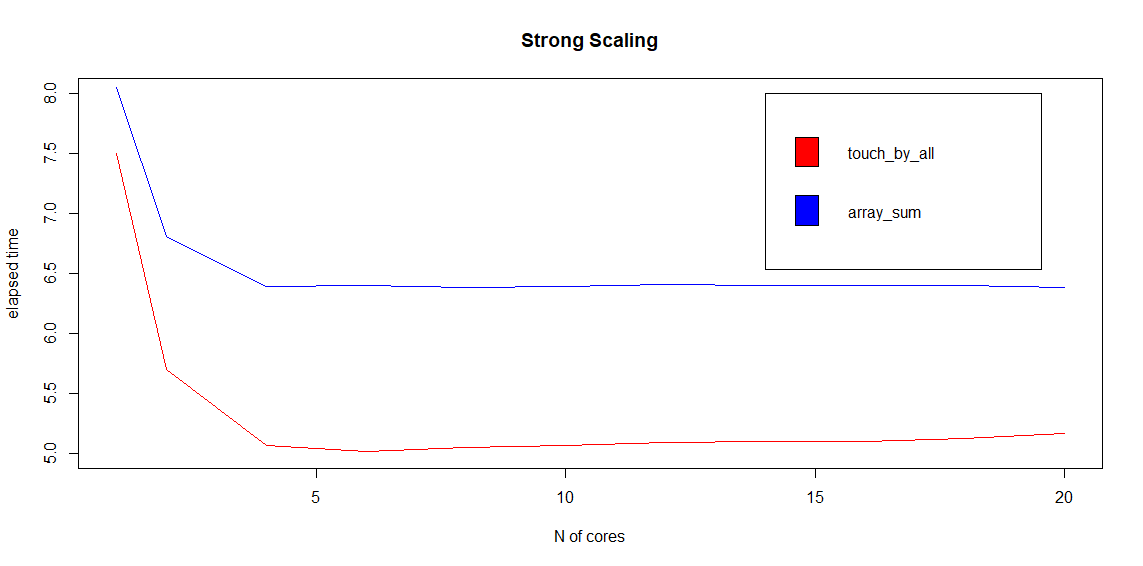
\includegraphics[width=0.8\columnwidth]{graphs/exercise_0_strongscaling} % Example image
	\caption{Elapsed times for $N=10^9$}
\end{figure}

\begin{figure}[H] % [h] forces the figure to be output where it is defined in the code (it suppresses floating)
	\centering
	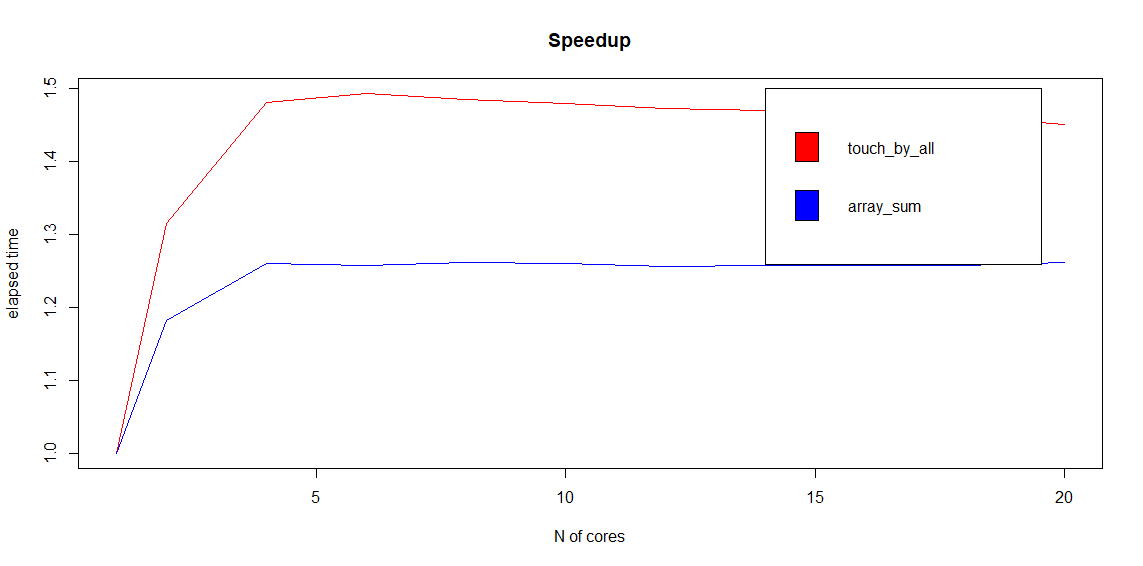
\includegraphics[width=0.8\columnwidth]{graphs/exercise_0_speedup} % Example image
	\caption{Speedup for $N=10^9$}
\end{figure}


We see that both codes scale and that the code that implements the touch-by-all policy is faster. The faster access to the cache memory saves time during the process, making touch\_by\_all.c a faster program.

\subsection{Parallel Overhead}
We will proceed our comparison by calculating the parallel overhead of the two programs. We can use the formula $ e(n,p) =\frac{\frac{1}{S_p(n,t)}-\frac{1}{p}}{1-\frac{1}{p}}$ to estimate the parallel overhead.  A plot with the measures we have would return:

\begin{figure}[H] % [h] forces the figure to be output where it is defined in the code (it suppresses floating)
	\centering
	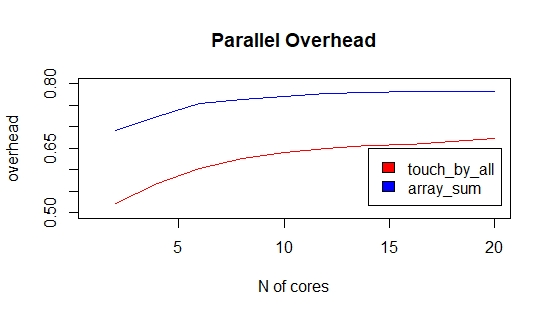
\includegraphics[width=0.8\columnwidth]{graphs/exercise_0_overhead} % Example image
	\caption{Overhead estimation for $N=10^9$}
\end{figure}
The touch\_by\_all code once again is better than the array\_sum code, since it has a lower parallel overhead.
But both lines are almost constant, showing that both codes have an almost constant parallel overhead while we increment the number of processors.

\subsection{Performance evaluation}
Now lets compare some valuable metrics for the two codes' executions:

\begin{adjustwidth}{-3cm}{}
\begin{tabular}[H]{l|l |l l l l| l l}
Metric & measures&&&&&mean&\\
CPU cycles& array\_sum &372889698& 143797361&671828181&373809554&390581199&-\\
          & touch\_by\_all&602487792&16412868&15030736&15901403&162458200&= \\
&&&&&&&	228122999\\				
					\hline
Cache misses & array\_sum&9459& 11492&49514&9484&19987.25&-\\
          & touch\_by\_all& 10356&10256 & 8417&12081&10277.5&=\\
&&&&&&&	 9709.75\\				
\hline
Elapsed time   & array\_sum& 0,014486573&0,007287606&0,024476034& 0,014344770&0.01514875&- \\
          & touch\_by\_all &0,021872540&0,002893806&0,002676134&0,002677902&0.007530096&=\\
					&&&&&&&	 0.00761865\\				
\hline
\end{tabular}
\end{adjustwidth}
Even if the single performances, measured with Perf, are quite similar in their randomness, we see that the touch\_by\_all code outperforms in average the array\_sum code in all the metrics. The most important metric is the cache misses, which decreases if a portion of the array is saved in each processor, which is the "touch by all" policy case.
\subsection{Conclusion}
The touch-by-all policy gives us a more performant code in terms of memory access and speed.
Once again we have found an optimization approach that exploits the cache's speed of access to speed up the execution time of the code.
%----------------------------------------------------------------------------------------
%	SECTION 3
%----------------------------------------------------------------------------------------

\section{Exercise 1}

We need to rewrite the code mpi\_pi.c by means of OpenMP directives. We had to solve all the problems we encountered in lesson, like avoiding race conditions and false sharing.
In the end we produced the simple code openmp\_pi.c that exploits thread parallelization to compute an estimate of pi based on a montecarlo geometrical approach.
\subsection{Strong and Weak Scalability}
We show the plots for the strong and weak scalability:


\begin{figure}[H] % [h] forces the figure to be output where it is defined in the code (it suppresses floating)
	\centering
	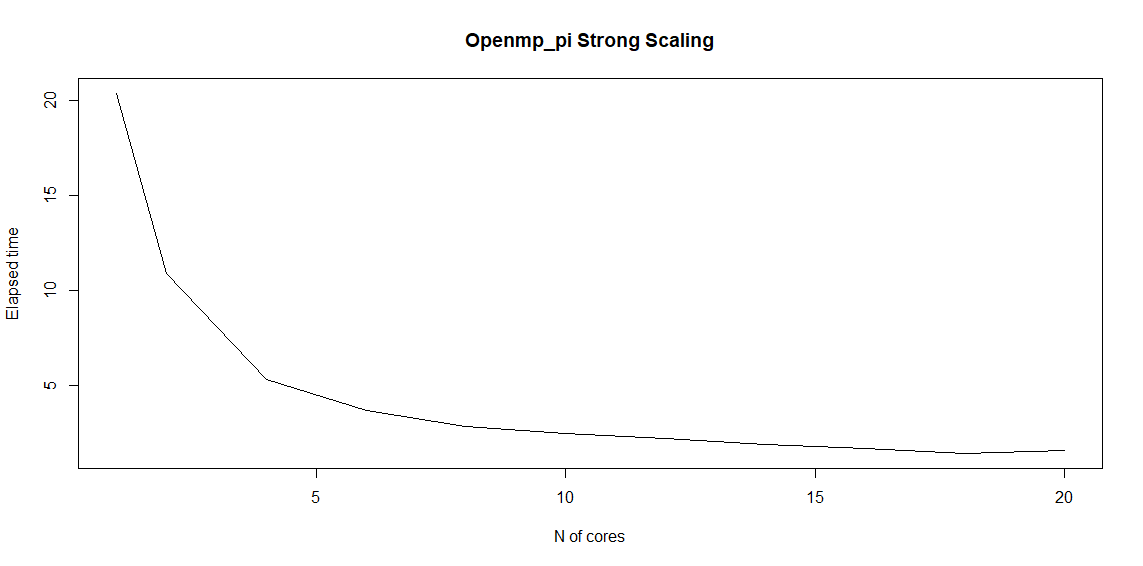
\includegraphics[width=0.8\columnwidth]{graphs/openmp_pi_strongscaling} % Example image
	\caption{Strong scaling test for $N=10^9$}
\end{figure}

\begin{figure}[H] % [h] forces the figure to be output where it is defined in the code (it suppresses floating)
	\centering
	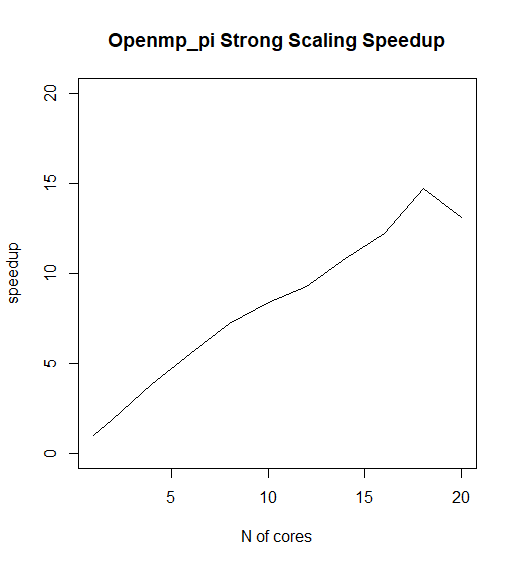
\includegraphics[width=0.8\columnwidth]{graphs/openmp_pi_strongscaling_speedup} % Example image
	\caption{Speedup for $N=10^9$}
\end{figure}

\begin{figure}[H] % [h] forces the figure to be output where it is defined in the code (it suppresses floating)
	\centering
	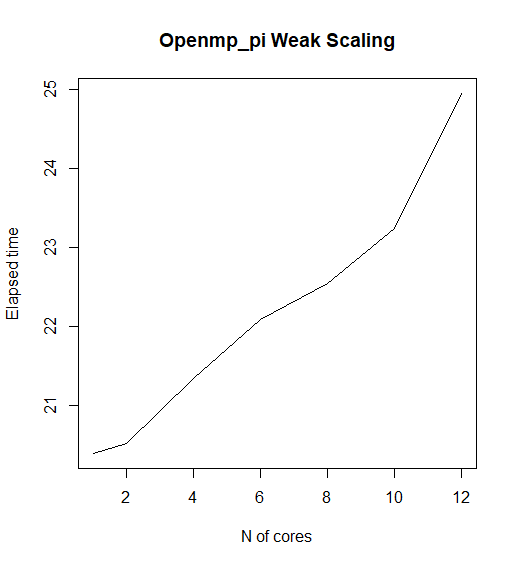
\includegraphics[width=0.8\columnwidth]{graphs/openmp_pi_weakscaling} % Example image
	\caption{Weak Scaling test for $N=10^4*P$}
\end{figure}

\begin{figure}[H] % [h] forces the figure to be output where it is defined in the code (it suppresses floating)
	\centering
	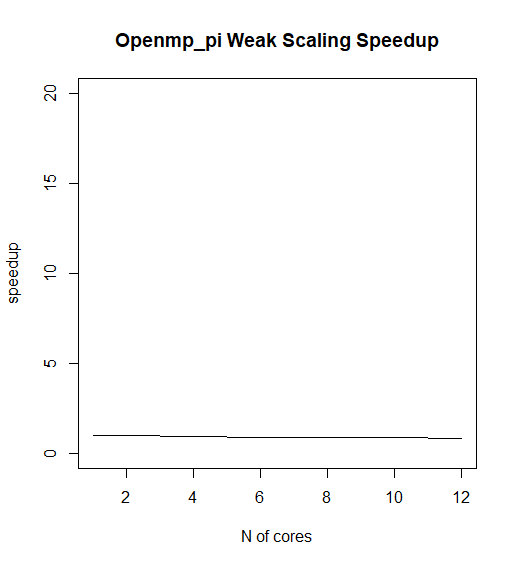
\includegraphics[width=0.8\columnwidth]{graphs/openmp_pi_weakscaling_speedup} % Example image
	\caption{Weak Scaling speedup for $N=10^4*P$}
\end{figure}
In the strong scalability setting the code scales very well, the speedup is almost linear. The weak scalability test also shows that the program handles well problems of increasing size through an increase of threads.
\subsection{Parallel overhead}

Now we estimate the parallel overhead, using again the formula to calulate $e(n,p)$ in the strong scaling context:


\begin{figure}[H] % [h] forces the figure to be output where it is defined in the code (it suppresses floating)
	\centering
	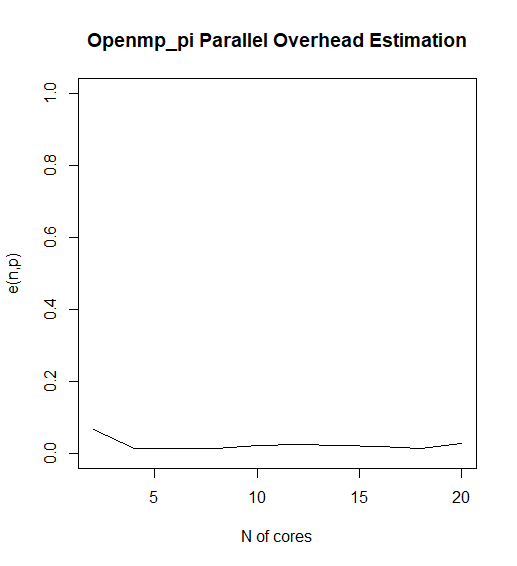
\includegraphics[width=0.8\columnwidth]{graphs/openmp_pi_strongscaling_overhead} % Example image
	\caption{Overhead estimate for $N=10^4*P$}
\end{figure}
We see that the overhead estimation remains almost constant, showing that the program's parallel overhead doesn't increase over the number of processors.
\subsection{Comparison with mpi\_pi.c}
Let's make some comparisons between the openMP version of the file and the MPI version.
As a first comparison we can plot the execution times of the two programs given a growing problem size and a fixed number of processors. Given 20 processors ,we run mpi\_pi.c on all processors, and then we run omp\_pi.c on 20 threads, one per processor. The plot is:

\begin{figure}[H] % [h] forces the figure to be output where it is defined in the code (it suppresses floating)
	\centering
	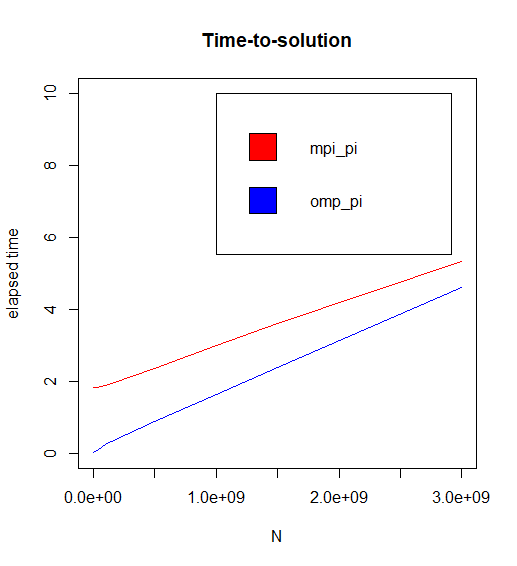
\includegraphics[width=0.8\columnwidth]{graphs/time_to_solution} % Example image
	\caption{Elapsed time for P =20}
\end{figure}
We see that omp\_pi.c is faster than mpi\_pi.c, even thought the fact that the message passing in mpi\_pi.c does some buffering(latency hiding) and thought the fact that there is an "atomic"' section in omp\_pi.c that introduces a serialization that slows down the program.
Now it's time to test the performance of mpi\_pi.c on a single node and on multiple nodes. We started with 1 node with 20 cores and we finished with 10 cores having 2 nodes each. We see if splitting processors on multiple nodes gives a slower execution time due to the network latency.

\begin{figure}[H] % [h] forces the figure to be output where it is defined in the code (it suppresses floating)
	\centering
	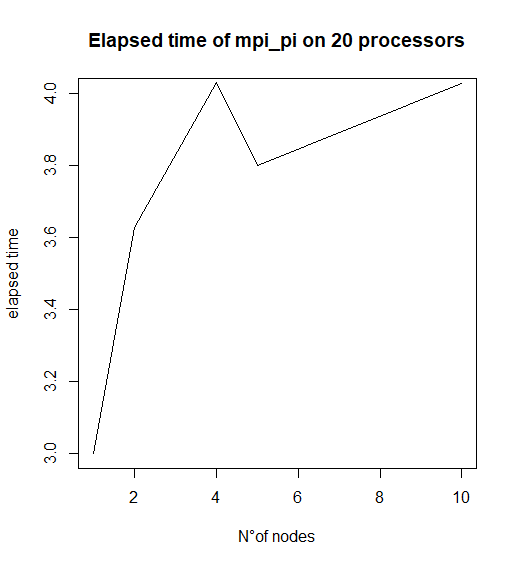
\includegraphics[width=0.8\columnwidth]{graphs/mpi_pi_elaps_time_on_nodes} % Example image
	\caption{Overhead for $N=10^4*P$}
\end{figure}

We see that the separation among nodes slows down the execution time in respect with the case of just one node. The openmp\_pi.c program running on 20 threads would instead have an elapsed time of 1.56 seconds, which is faster. The inter-core communication is faster than inter-node communication.
We can then compare the portions of the codes that have the same function.
There are two portions of interest: the initialization and the identification of the points that belong inside the circle and the consequent partial sum of such points, and then there is the full summation of those partial sums. These two portions are critical in the two codes.
The first portion is parallelized in both codes, so it could be seen as a parallelization comparison.
The execution time for the first portion is the following:

\begin{figure}[H] % [h] forces the figure to be output where it is defined in the code (it suppresses floating)
	\centering
	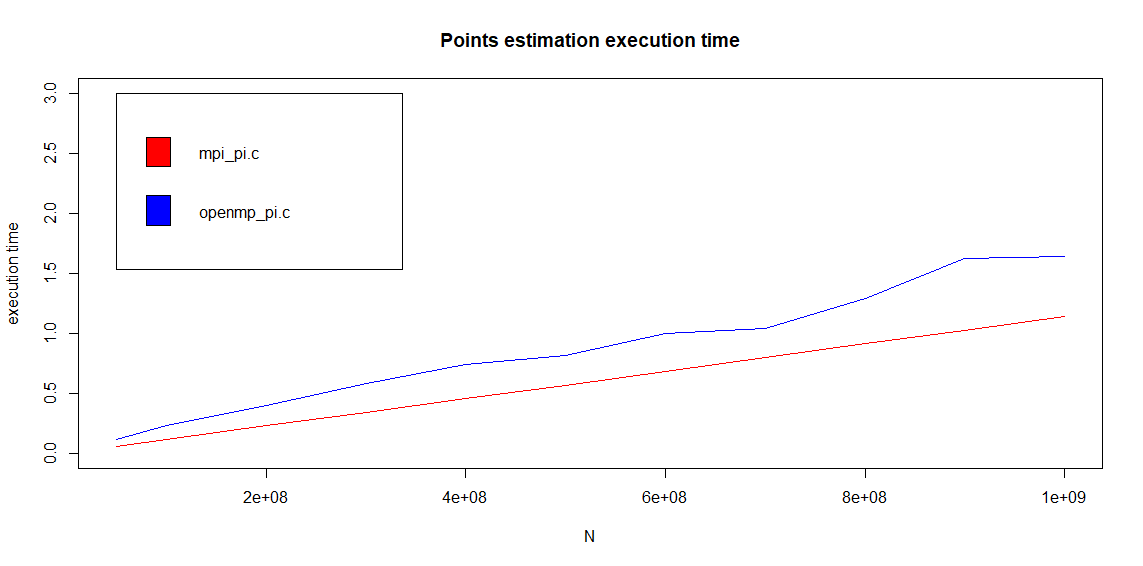
\includegraphics[width=0.9\columnwidth]{graphs/pi_points_estimation_execution_time.png} % Example image
	\caption{Execution time for a growing $N$}
\end{figure}

We see that, in contrast with the other graph, that openmp\_pi.c has a slower execution time.
This points out the fact that mpi\_pi.c has a higher overhead than openmp\_pi.c that slows down the total execution time.
Now we see that the second portion of the code has two similar implementations in mpi\_pi.c and openmp\_pi.c.
In mpi\_pi.c the total sum of the results from each processor is carried out thanks to message passing. The master node fetches the partial sums from each slave processor.
 In openmp\_pi.c the total sum is carried out thanks to a serialization due to the parallel atomic directive.
In both cases we have the sequential participation of each parallel process to the resulting summation.
We see that this portion of the code has an execution time given by: 
\begin{figure}[H] % [h] forces the figure to be output where it is defined in the code (it suppresses floating)
	\centering
	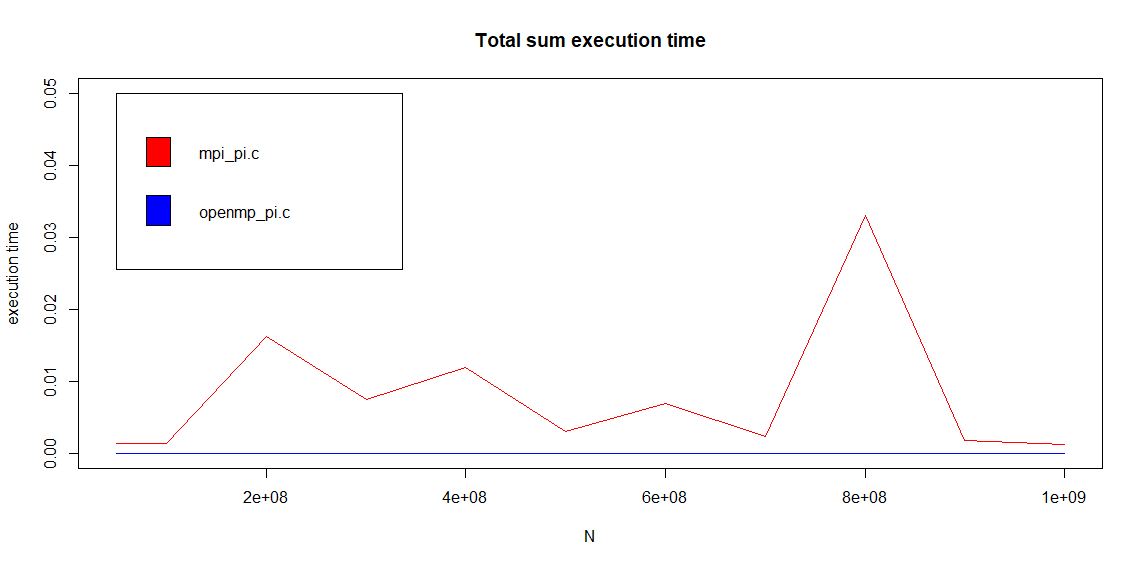
\includegraphics[width=0.9\columnwidth]{graphs/pi_total_sum_execution_time} % Example image
	\caption{Execution time for a growing $N$}
\end{figure}

We see that the execution of the second portion of the code is way faster in the OpenMP version of the code. 
Since in both codes there is still a sequential access from the parallel threads/processors we can clearly identify the cause of this difference in the overhead introduced by the send and receive functions.

We plot here the sum of the times of the two portions of the code:
\begin{figure}[H] % [h] forces the figure to be output where it is defined in the code (it suppresses floating)
	\centering
	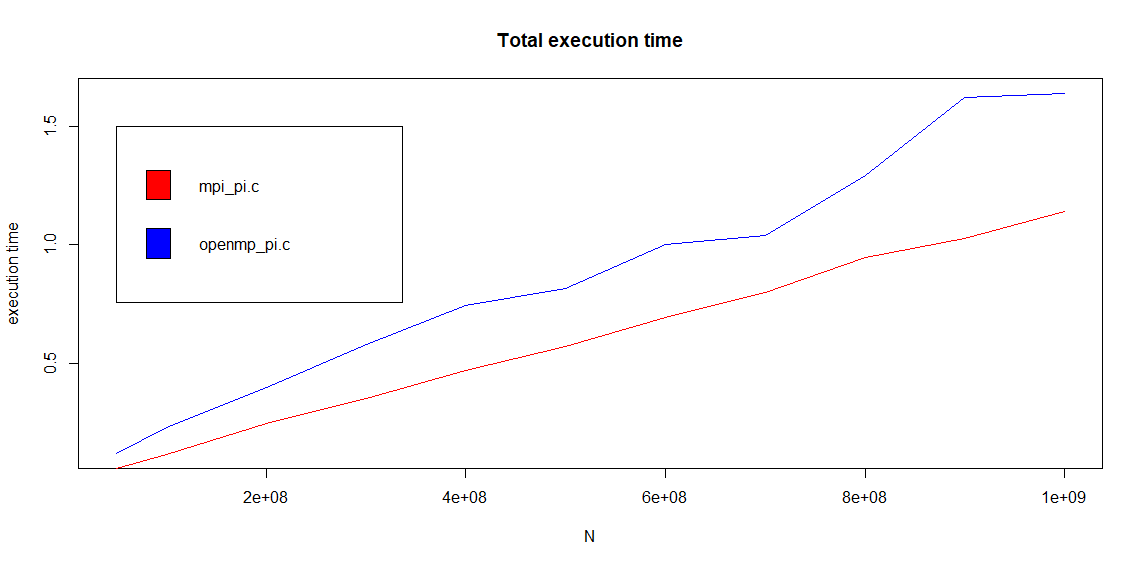
\includegraphics[width=0.9\columnwidth]{graphs/pi_total_execution_time} % Example image
	\caption{Sum of the execution times for a growing $N$}
	\label{fig:execution_time_total_graph}
\end{figure}

Now we have the elapsed time for both programs, and we have the walltime for both programs.
We can estimate the parallel overhead of both codes by subtracting the walltime from the execution time:

\begin{figure}[H] % [h] forces the figure to be output where it is defined in the code (it suppresses floating)
	\centering
	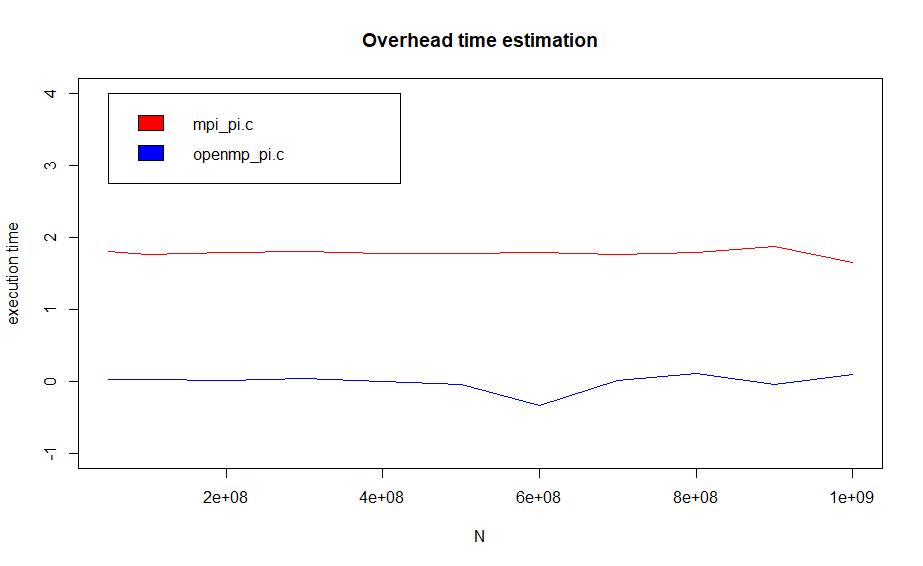
\includegraphics[width=0.9\columnwidth]{graphs/final_overhead.png} % Example image
	\caption{Overhead times estimation for a growing $N$}
	 \label{fig:overhead_graph}
\end{figure}
Here we see again that mpi\_pi.c has a higher overhead than openmp\_pi.c. We also see that openmp\_pi.c's overhead is again constant.In the previous plot the overhead has been calculated on the parallel speedup of the strong scaling test, while here we are instead increasing the problem size.
We see that there is some noise in the measurement and that the graph of openmp\_pi.c's overhead estimation is mostly negative.
This is due to the truncation error on the value taken from /usr/bin/time because of the small difference between elapsed time and walltime (that can be seen by outputting all the variables containing the results of /usr/bin/time and omp\_get\_Wtime() and on the graph below).

\begin{figure}[H] % [h] forces the figure to be output where it is defined in the code (it suppresses floating)
	\centering
	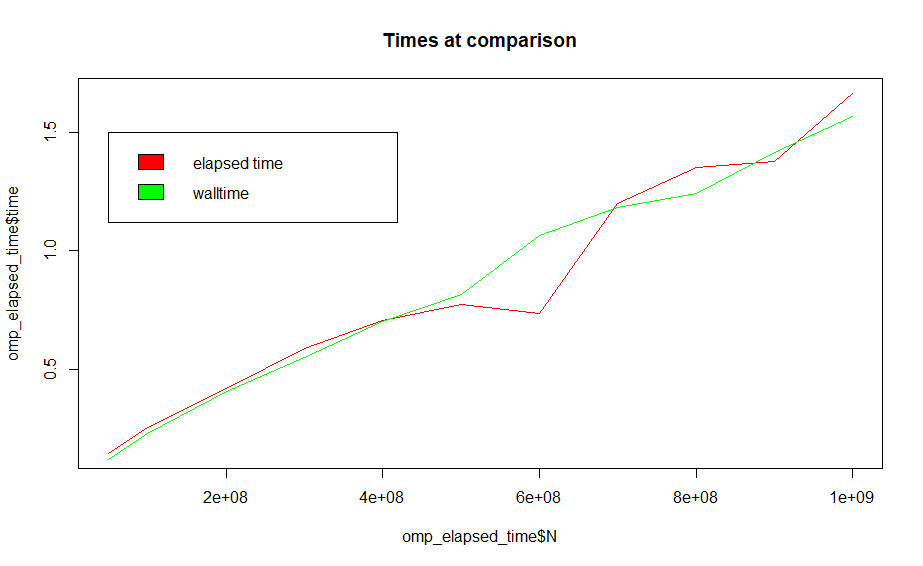
\includegraphics[width=0.9\columnwidth]{graphs/times_comparison_openmp_pi.png} % Example image
	\caption{execution times comparison for a growing $N$}
\end{figure}


We can still conclude that the parallel overhead of openmp\_pi.c is relatively small and also constant, much like the e(n,t) estimate. The second estimate we did in Figure~\ref{fig:overhead_graph} is useful to show that mpi\_pi.c has a bigger parallel overhead than openmp\_pi.c.

\subsection{Strong scalability comparison}
We can obtain the same results in a strong scalability test.
We plot the elapsed time and the walltime for both codes. The distance between the two graphs represents the overhead estimate:
\begin{figure}[H] % [h] forces the figure to be output where it is defined in the code (it suppresses floating)
	\centering
	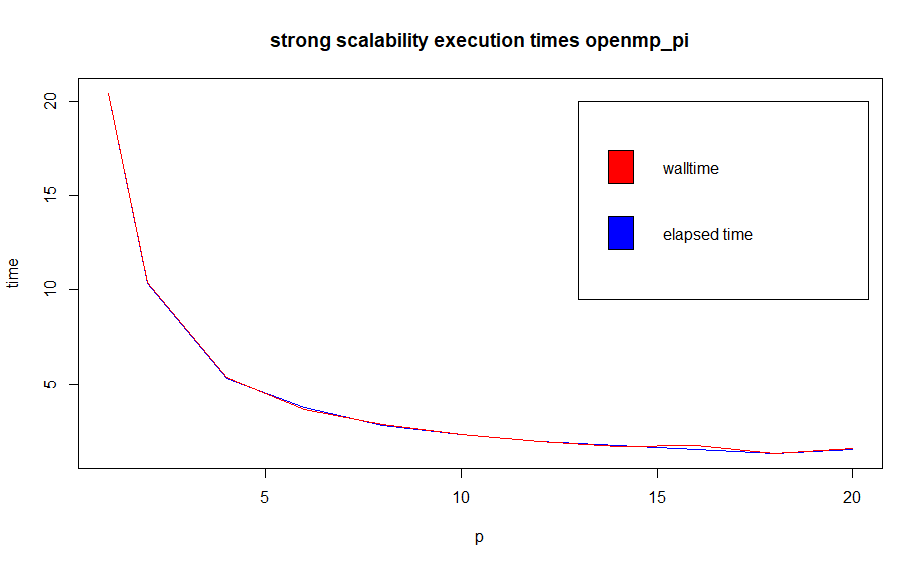
\includegraphics[width=0.9\columnwidth]{graphs/strong_scaling_times_comparison_openmp.png} % Example image
	\caption{execution times comparison for $N=1000000000$}
\end{figure}
\begin{figure}[H] % [h] forces the figure to be output where it is defined in the code (it suppresses floating)
	\centering
	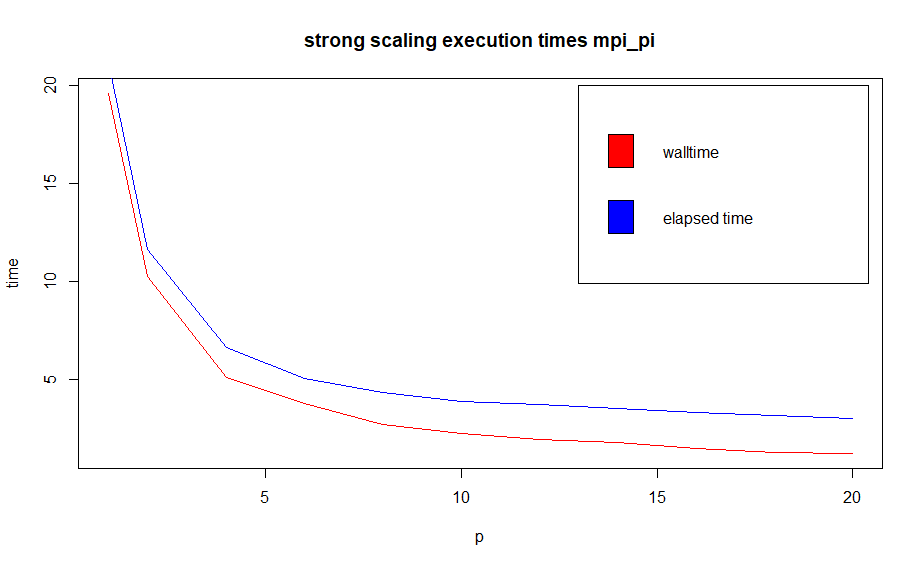
\includegraphics[width=0.9\columnwidth]{graphs/strong_scaling_times_comparison_mpi.png} % Example image
	\caption{execution times comparison for $N=1000000000$}
\end{figure}
In the second plot there is a larger difference between walltime and elapsed time, showing once again that mpi\_pi\_pi.c has a bigger overhead than openmp\_pi.c.

We plot now both the previous graphs on the same graph:
\begin{figure}[H] % [h] forces the figure to be output where it is defined in the code (it suppresses floating)
	\centering
	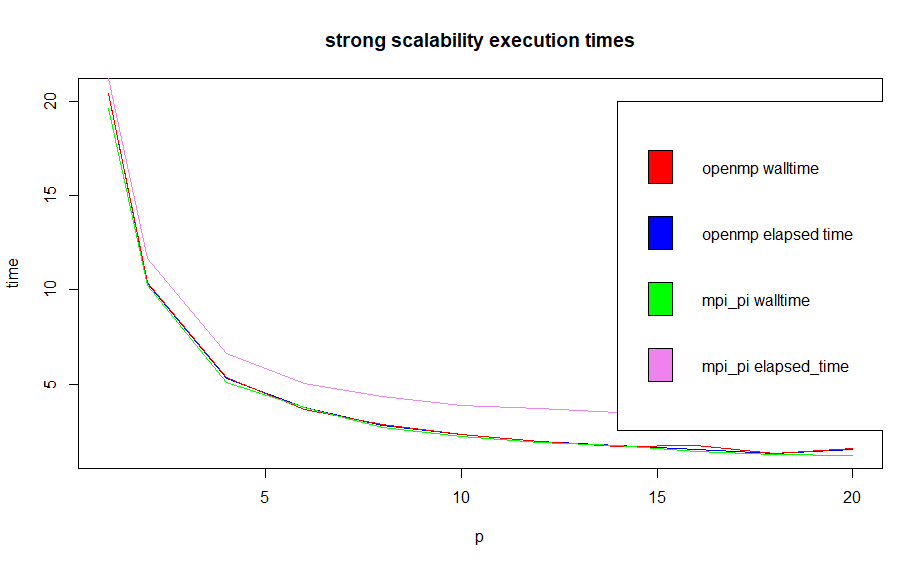
\includegraphics[width=0.9\columnwidth]{graphs/strong_scaling_times_comparison.png} % Example image
	\caption{execution times comparison for $N=1000000000$}
\end{figure}
Here once again we see that the two walltimes are comparable, while mpi\_pi.c's walltime is a little faster than openmp\_pi.c's walltime(as we saw in the previous figure \ref{fig:execution_time_total_graph}), and that mpi\_pi.c's elapsed time execution is longer. 
\subsection{Conclusion}
In conclusion we can say that the MPI version of the code has a faster execution of the script, but its parallel overhead makes the code slower than the OpenMP version, as we have seen by comparing the walltimes with the elapsed times. 

 We have seen that the overhead estimation of the MPI version has a flat and non-negligible graph  with respect to the OpenMP version of the code, where the overhead is flat and negligible. Figure \ref{fig:overhead_graph} proves our point.

%----\begin{figure}[H] --\begin{figure}[H] % [h] forces the figure to be output where it is defined in the code (it suppresses floating)----------------------------------------------------------------------------------
%	SECTION 4
%----------------------------------------------------------------------------------------
%----------------------------------------------------------------------------------------
%	SECTION 5
%----------------------------------------------------------------------------------------



%----------------------------------------------------------------------------------------
%	SECTION 6
%----------------------------------------------------------------------------------------


%----------------------------------------------------------------------------------------
%	BIBLIOGRAPHY
%----------------------------------------------------------------------------------------
%---------------------------------------------------------------------------------------


\end{document}